%%%%%%%%%%%%%%%%%%%%%%%%%%%%%%%%%%%%%%%%%%%%%%%%%%%%%%%%%%%%%%%%%%%%%%%%%%%%% 
%
% This is a LaTeX file for an A3 poster.
%
%%%%%%%%%%%%%%%%%%%%%%%%%%%%%%%%%%%%%%%%%%%%%%%%%%%%%%%%%%%%%%%%%%%%%%%%%%%%% 

%%%%%%%%%%%%%%%%%%%%%%%%%%%%%%%%%%%%%%%%%%%%%%%%%%%%%%%%%%%%%%%%%%%%%%%%%%%%% 
%%%%%%%%%%%%%%%%%%%%%%%%%%%%%%%%%%%%%%%%%%%%%%%%%%%%%%%%%%%%%%%%%%%%%%%%%%%%%
%
% Asymptotic behavior of solutions to the generalized Becker-Döring
% equations for general initial data.
%
% Poster for the HYKE-3 meeting in Rome, 13-15 April 2005.
% 
%%%%%%%%%%%%%%%%%%%%%%%%%%%%%%%%%%%%%%%%%%%%%%%%%%%%%%%%%%%%%%%%%%%%%%%%%%%%%
%%%%%%%%%%%%%%%%%%%%%%%%%%%%%%%%%%%%%%%%%%%%%%%%%%%%%%%%%%%%%%%%%%%%%%%%%%%%%

\documentclass{article}
% To modify the size of the page:
\usepackage[dvips,a3paper,landscape,centering,margin=2cm]{geometry}
\usepackage{multicol}
\usepackage[utf8]{inputenc}
\usepackage[svgnames]{xcolor}
\usepackage{url}
\usepackage{hyperref}
\usepackage{multirow}
\usepackage{amsmath, amsthm, amsfonts}
\usepackage{graphicx}           % Include figure files.
\usepackage{subcaption}
% Colors
% -------
\definecolor{azulillo}{rgb}{0.8,0.85,1}
\definecolor{marronrp3}{rgb}{.9,.9,.7}
\definecolor{salmon}{rgb}{1,.9,.8}
\definecolor{rojo}{rgb}{.6,.1,0}

\pagestyle{empty}

\def\to{\rightarrow}

% Hyphenation
\hyphenation{coa-gu-la-tion frag-men-ta-tion}

% ===========================================================================

\title{}
\author{}
\date{}

\begin{document}
%\maketitle

\begin{center}
  \begin{minipage}{.19\linewidth}
    
\includegraphics[width=0.3\linewidth]{figures/tuc_logo.png}

\includegraphics[width=0.3\linewidth]{figures/IIT_logo.png}

\includegraphics[width=0.3\linewidth]{figures/auth_logo.jpg}
  \end{minipage}
  %&
  \begin{minipage}{.6\linewidth}
    \begin{center}
      \Huge \color{DarkGreen} \textbf{A Realistic Dataset Generator for Smart Grid Ecosystems
with Electric Vehicles}\\\vspace{10pt}
\large \color{Black} \textbf{Georgios Charalambidis$^{1}$, Charilaos Akasiadis$^{2}$, Emmanouil S. Rigas$^{3}$ and Georgios Chalkiadakis$^{1}$}\\[0.2cm] % Author(s)
\small 1. School of Electrical \& Computer Engineering, Technical University of Crete, Greece\\[0.1cm] % University
\small 2. Institute of Informatics \& Telecommunications,
NCSR ``Demokritos'', Greece\\[0.1cm] %
\small 3. School of Medicine,
Aristotle University of Thessaloniki, Greece\\[0.1cm] %Affiliation 2
\small \texttt{GitHub repository: \url{https://github.com/tuc-intelligence-energy/smartgrid-dataset-generator}}\\
    \end{center}
  \end{minipage}
  %&
  \hspace{.03\linewidth}
  \begin{minipage}{0.16\linewidth}
    \begin{flushright}
      
\includegraphics[scale=2,width=\linewidth]{figures/eenergy2022-logo.png}
\hspace{1cm}
    \end{flushright}
  \end{minipage}
\end{center}

\vspace{.1cm}

% ---------------------------------------------------------------------------

\setlength{\columnsep}{1cm}



\begin{multicols}{3}
%\vspace{-10cm}
\noindent
%\begin{minipage}[t]{\linewidth}
\noindent
\fcolorbox{black}{Lavender}{
  \begin{minipage}[t]{\linewidth}
    \vspace{.05cm}
    \begin{center}
      \vspace{.1cm}
      \section*{\Large Motivation}
    \end{center}
%    \begin{itemize}
    \hspace{0.1cm}$\bullet$ The Electric Vehicles market is rapidly expanding -- different geographical regions have different characteristics.\\
    \hspace{0.1cm}$\bullet$ We need to test and verify methods for optimization, scheduling, pricing, etc. using real data.\\
   \hspace{0.1cm}$\bullet$ Privacy issues hinder researchers' access to data.\\
    \hspace{0.1cm}$\bullet$ Dataset generators must be realistic and privacy preserving.\\
%\end{itemize}
\underline{Our solution}:\\
    \hspace{0.1cm}$\circ$ We incorporate several anonymized datasets.\\
    \hspace{0.1cm}$\circ$ We put forward generation mechanisms that fit to the existing data and produce new, that is different in absolute values, but adhere to the statistics and principles of the original.\\
    \hspace{0.1cm}$\circ$ Four methods to compare and select based on user needs.\\
    \hspace{0.1cm}$\circ$ Additional smoothing and summarization and visualization capabilities.\\
    \hspace{0.1cm}$\circ$ Data for microgrid level generation, consumption, and EV usage.\\
     \hspace{0.1cm}$\circ$ Configurable constraints for consistency control
  \end{minipage}} %\hfill\vfill
%\begin{minipage}[b]{0.6\linewidth}
%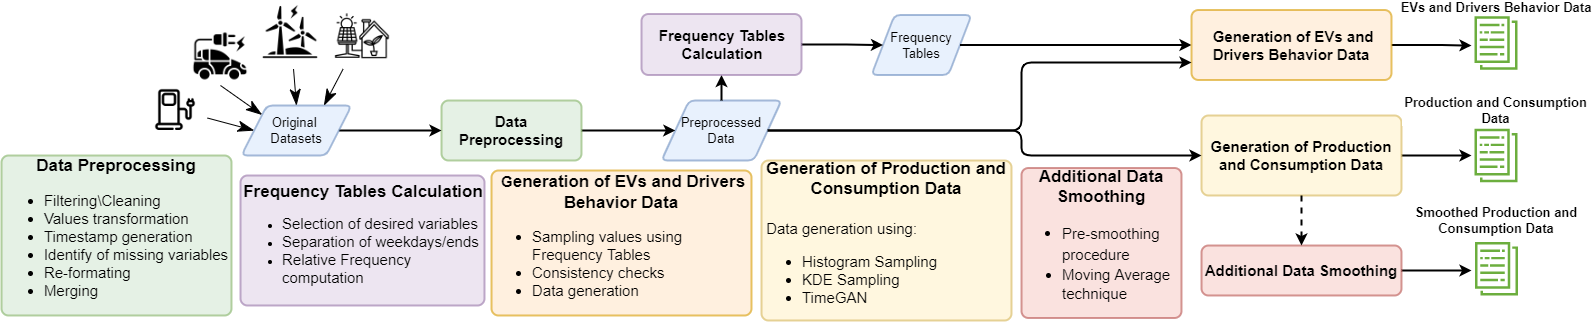
\includegraphics[width=\textwidth]{figures/overview_arch.png}
%\end{minipage}
%\end{minipage}

\vspace{.3cm}
\section*{Input Data}
Data related to EV comes from many different publicly available sources:\\ 
$\mbox{     }$\\
Characteristics of EVs and Chargers: \\ \indent {\em ``Mendeley Data platform'', ``Spirit Energy'', ``Tesla''}  \\ %\footnote{`Dataset of electric passenger cars with their specifications', \url{https://data.mendeley.com/datasets/tb9yrptydn/2}.} 
$\mbox{     }$\\
Drivers Behavior: \\\indent{\em ``My Electric Avenue''}\\
$\mbox{     }$\\
Aggregate generation levels per production type, as well as aggregate demand for all European regions for the recent years: \\\indent{\em ``ENTSOE Transparency Platform''}\\ 

\vspace{-.5cm}

\section*{Preprocessing}
As the original data has different formats, we need to apply specific transformations, and then combine it properly in order to end up with the final input files. As a first step of the generation process, we preprocess the acquired data files to assign them appropriate timestamps  
consistent across all generated files, i.e., \emph{Date, Year, MonthOfYear, DayOfWeek, TimeOfDay}.
Regarding the data related to the trip events, the file has the same format as that of the charging events: each row represents a trip event/action and each column, the exact time of a trip event, the duration of the trip, the trip distance and the power consumed during each trip respectively. 
%By extension, we followed similar techniques in order to pre-process the data. 
%We converted the start and end dates of the trip events into the appropriate format and used them to calculate the duration of each event (in minutes), in a new column called \emph{TripTime}. Lastly, we calculate the velocity of the vehicles through a simple time-distance relationship, assuming that the vehicle performs linear motion with constant speed.

%In terms of the generated synthetic data output files (\emph{EVs and Drivers Behavior Data} in Figure~\ref{fig:dataflow} and Table~\ref{tab:dataInfo}), their number is proportional to the number of drivers that the user has specified. %as a configuration. 
%For each one, the number of rows corresponds to measurements for a particular time interval, and each column represents the characteristics of each driver's EV, detailed information about charging events 
%%(i.e., exact time of charging event, duration of charge and status of the battery)
%and the characteristics of the charger with which a charging event takes place.
%%(i.e., AC or DC, single-phase or 3-phase, charger’s charging speed and rated power)
%Finally, detailed information on trip events are provided.
%(i.e., exact time of a trip event, the duration of a trip, the distance travelled and the power consumed during each trip).
%In addition, since the columns of the output files refer to both charging and trip events, in case of a charging event the columns related to the trip event are empty and vice versa. If neither event takes place, all  aforementioned columns are left empty.

For the other data category, energy production and total consumption, we convert the timestamp to the appropriate format and combine measurements into a common file.
A new column is inserted, that holds the imbalance between the aggregates of consumption and production. 
%A resulting positive number indicates that energy is imported from neighbouring regions; otherwise, it is exported.
%while this data can easily be augmented with additional information from other sources. 
%The combination of these two data sources
%is used to construct a second CSV file 
%provides information regarding EV technical characteristics, such as the equipped battery specification and the overall energy consumption of the EV.
%Here, the number of rows corresponds to different EV models, and the number of columns to the various characteristics
%Information about the different types of the available chargers (AC or DC, Regular socket, Single phase, or 3 phases),  charging speed and rated power is based on the``Spirit Energy'' website.
% A different input CSV file, produced during preprocessing, is used to dictate the specifications of the available chargers, based on the``Spirit Energy'' website, %\footnote{\url{https://www.spiritenergy.co.uk/kb-ev-understanding-electric-car-charging}} 
% and it contains the different types of chargers (AC or DC, Regular socket, Single phase, or 3 phases), their charging speed and their rated power.

%Finally, the data related to the drivers' driving behavior comes from the ``My Electric Avenue'' project. %\footnote{\url{https://eatechnology.com/resources/projects/my-electric-avenue/}} 
%There,  participants monitored the usage of over 200 EVs, a number of low voltage networks, and the switching of the EVs to support those networks. The trial participants’ charging and driving behavior was recorded using the EVs’ telematics systems. We utilize two files from that project: the first one contains information about the times each EV charged, as well as the state of charge for each time an EV is connected and charged; and the second one, contains distance, times, and power consumption information for each of the recorded drivers' trips.
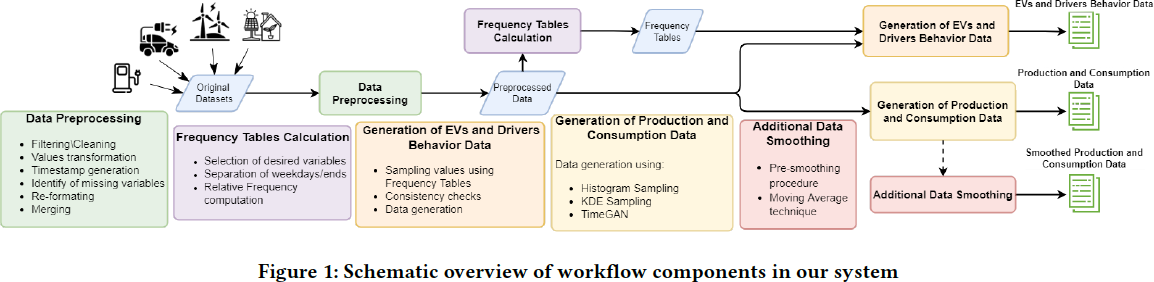
\includegraphics[width=0.65\textwidth]{figures/overview.png}
%\captionof{figure}{{\bf Method Overview}}

% % \begin{table}[h]
% %     \caption{Description of input and output data}
% %     \label{tab:dataInfo}
\vspace{-1.5cm}
\section*{Data Generation Techniques}
\vspace{-0.5cm}
Our dataset generation process uses different statistical methods to produce synthetic data.
There are two desired types of data to generate: 
\hspace{0.1cm}$\circ$ Energy Consumption and Production, 
\hspace{0.1cm}$\circ$ EVs and Drivers Behavior data. 
We adopt three different generation methods that can be used interchangeably:\\
\indent \hspace{0.1cm}$\circ$ {\em Histogram Sampling} , {\em KDE Sampling} , {\em TimeGAN}\\
Since the drivers' 
%driving 
behavior data %, which 
do not come in a time series format, the application of these methods is not meaningful. Therefore, we also put forward a {\em Frequency Tables Method}, which requires no such assumption for the input. 

\vspace{-1.2cm}
\section*{Results}
\vspace{-.5cm}
\noindent         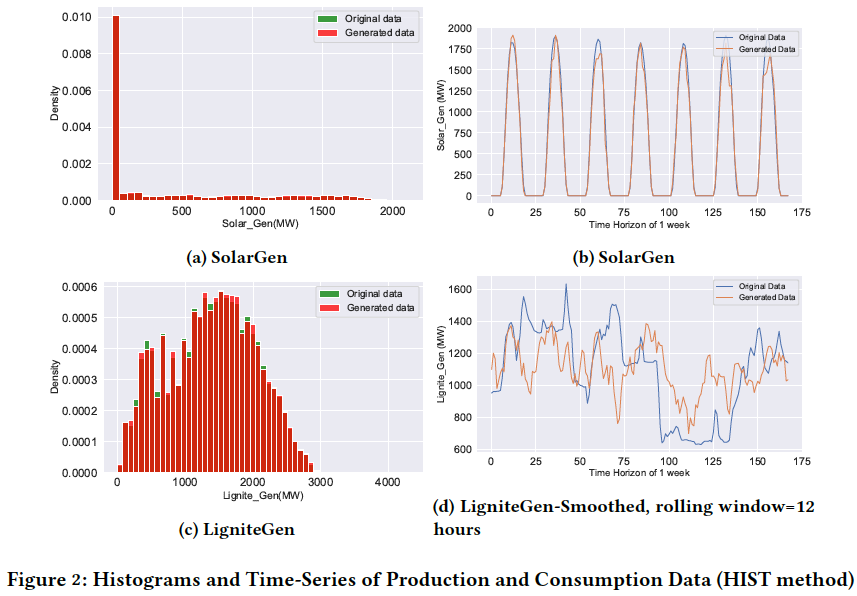
\includegraphics[width=\linewidth]{figures/hist-c}

\vspace{3cm}
%\vspace{7cm}
$\mbox{     }$\\
$\mbox{     }$\\
$\mbox{     }$\\
$\mbox{     }$\\
$\mbox{     }$\\
$\mbox{     }$\\
$\mbox{     }$\\
$\mbox{     }$\\
$\mbox{     }$\\
$\mbox{     }$\\
$\mbox{     }$\\
$\mbox{     }$\\
$\mbox{     }$\\
$\mbox{     }$\\
$\mbox{     }$\\
$\mbox{     }$\\
\addtocounter{figure}{+2}
\noindent         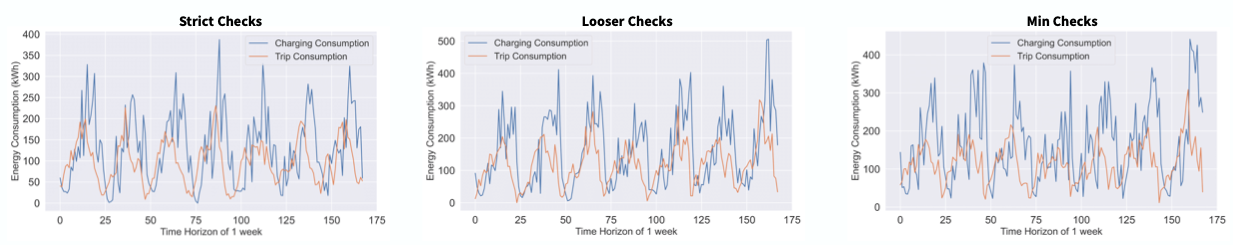
\includegraphics[width=\linewidth]{figures/data}
\captionof{figure}{{\bf EV Consumption}}

\vspace{.5cm}
\noindent         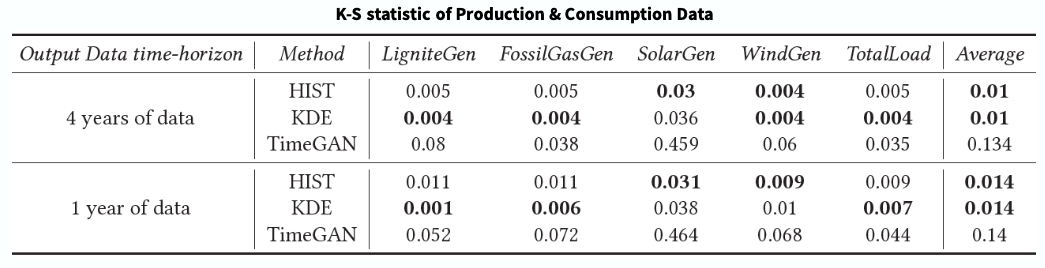
\includegraphics[width=\linewidth]{figures/table1}

\vspace{.5cm}
\noindent         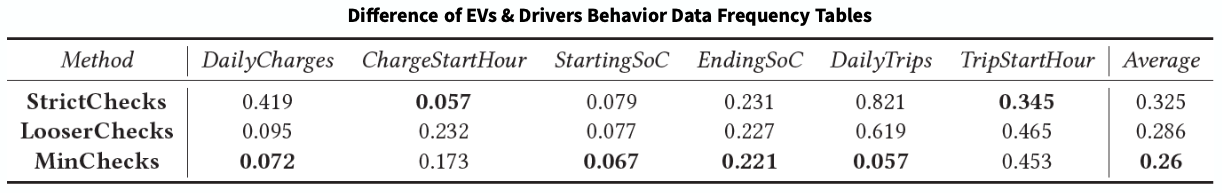
\includegraphics[width=\linewidth]{figures/table}
%\begin{table}
%    \caption{Difference of Drivers Behavior Data Frequency Tables}
%    \label{tab:metricsEV}
%    \begin{tabular}{c|cccccc|c}
%    \textit{Method} & \textit{DailyCharges} & \textit{ChargeStartHour} & \textit{StartingSoC} & \textit{EndingSoC} & \textit{DailyTrips} & \textit{TripStartHour} & \textit{Average} \\ 
%    \textbf{StrictChecks} & 0.419 & \textbf{0.057} & 0.079 & 0.231 & 0.821 & \textbf{0.345} & 0.325 \\
%    \textbf{LooserChecks} & 0.095 & 0.232 & 0.077 & 0.227 & 0.619 & 0.465 & 0.286 \\
%    \textbf{MinChecks} & \textbf{0.072} & 0.173 & \textbf{0.067} & \textbf{0.221} & \textbf{0.057} & 0.453 & \textbf{0.26} \\ 
%    \end{tabular}
%\end{table}
%\vspace{30cm}
\section*{Future Work}

In terms of future work, we aim to evaluate the application of
additional data analysis techniques for datasets that exhibit some
periodicity in their values; and at the same time, to explore ways to
more accurately simulate data that does not appear to be periodic.
Additionally, our dataset generator
could also serve as a tool towards the verifiability of various multiagent
systems. Finally,
we intend to extend our dataset generator to cover the V2G mode
of EV operation, which is crucial for the efficient integration of
renewables into the Grid.
%{\textcolor{rojo}{The generalized Becker-Döring system is the special
%    case where $a_{jk}$ and $b_{jk}$ are zero whenever $\min\{j,k\} >
%    N$ for some $N$. For $N=1$ the system is the Becker-Döring
%    system.}  }

%\section*{Asymptotic Behavior}
%
%The study of the long-time behavior of solutions to these equations is
%expected to be a model of physical processes such as phase transition.
%Under certain general conditions which include a detailed balance we
%can ensure the existence of equilibrium states. In these conditions,
%there is a critical mass $\rho_s \in ]0,\infty[$ such that any
%solution that initially has mass $\rho_0 \leq \rho_s$ will converge
%for large times, in a certain strong sense, to an equilibrium solution
%with mass $\rho_0$. On the other hand, any solution with mass above
%$\rho_s$ converges (in a weak sense) to the only equilibrium with mass
%$\rho_s$; this weak convergence can then be interpreted as a phase
%transition in the physical process modelled by the equation.
%
%Convergence in this weak sense means that a fixed part of the total
%mass of particles is found to be forming larger and larger clusters as
%time passes and the mean size of clusters goes to infinity. The
%physical interpretation of this, depending on the context, can be a
%change of phase or the apparition of crystals, for example.
%
%\noindent
%\begin{center}
%  \noindent
%  \colorbox{marronrp3}{
%    \begin{minipage}[t]{.96\linewidth}
%      \begin{align*}
%        & \text{\Large Below critical mass}
%        &\to \quad
%        &\begin{cases}
%          \text{ \Large Trend to equilibrium }\\
%          \text{ \Large Strong convergence }
%        \end{cases}
%        &
%        \\
%        &\text{\Large Over critical mass }
%        &\to \quad
%        &\begin{cases}
%          \text{ \Large Large clusters created}\\
%          \text{\Large Weak convergence }
%        \end{cases}
%        &
%      \end{align*}
%    \end{minipage}
%  }
%\end{center}
%
%\begin{center}  
%
%\vspace{.5cm}
%
%\Large
%\begin{tabular}[t]{c|c}
%  \multicolumn{2}{c}{\huge \textbf{Previous results}}
%  \vspace{.3cm}
%  \\
%  Becker-Döring& Ball, Carr, Penrose\\
%  system       & \cite{BCP86,BC88} (1986-88)\\
%  \hline
%  Generalized Becker-Döring &Carr, da Costa\\
%  (rapidly decaying initial data) &\cite{CdC94} (1994)\\
%  \hline
%  Generalized Becker-Döring & da Costa \\
%  (small initial data) & \cite{dC98} (1998)
%\end{tabular}
%\end{center}
%
%
%% ---------------------------------------------------------------------------
%
%\section*{Sketch of the proof}
%
%Our proof is a generalization of a method used in unpublished notes by
%Ph. Lauren\c{c}ot and S. Mischler \cite{LM}, inspired by the proof of
%uniqueness of solutions to the Becker-D\"oring equation in
%\cite{LM02e}.
%
%It is known that, under common assumptions, \emph{there is always} at
%least weak convergence to a certain equilibrium state;
%\textcolor{rojo}{the problem reduces to show that for an initial
%  density under the critical one solutions converge \emph{strongly} to
%  the equilibrium \emph{with the same density}}. To prove this, it is
%enough to show that the tails of the solutions are small enough, so
%that strong convergence holds. The following estimate, roughly stated
%here, is the key of our proof:
%
%\noindent
%\colorbox{marronrp3}{
%  \begin{minipage}[t]{.96\linewidth}
%    \vspace{.2cm}
%    \centerline{\huge \textbf{Main estimate}}
%    \vspace{.05cm}
%
%    \Large
%    If $c = \{c_j\}_{j \geq 1}$ is a solution to the generalized
%    Becker-Döring equations with density below the critical one, then
%    there is some sequence $r_i$ (which tends to zero as $i \to
%    \infty$) such that the tails of the solution have mass below
%    $r_i$; this is,
%    \begin{equation*}
%      \sum_{k=i}^\infty k c_k(t) \leq r_i
%    \end{equation*}
%    for all times $t$ after some time $t_0$.
%    \\\hspace{.05cm}
%  \end{minipage}
%}
%
%\vspace{.5cm}
%
%The proof of this consists mainly of an estimate obtained by
%differentiating the quantity $H_i := (G_i-r_i)_+$ (the positive part
%of $G_i - r_i$), proving with a differential inequality that it must
%remain zero for all times starting from a certain $t_0$.
%% ---------------------------------------------------------------------------
%%
%\small
%\begin{thebibliography}{}
%
%\bibitem{BCP86} J. M. Ball, J. Carr, O. Penrose, \emph{The
%    Becker-D\"oring cluster equations: basic properties and asymptotic
%    behaviour of solutions}, Comm. Math. Phys. 104, 657--692 (1986)
%
%\bibitem{BC88} J. M. Ball, J. Carr, \emph{Asymptotic behaviour of
%    solutions to the Becker-D\"oring equations for arbitrary initial
%    data}, Proc. Roy. Soc. Edinburgh Sect. A, 108, 109-116 (1988)
%
%\bibitem{C04} J. A. Cañizo, \emph{Asymptotic behavior of solutions to
%    the generalized Becker-Döring equations for general initial data},
%  preprint.
%
%\bibitem{CdC94} J. Carr, F. P. da Costa, \emph{Asymptotic behaviour of
%    solutions to the coagulation-fragmentation equations. II. Weak
%    fragmentation}, J. Stat. Phys. 77, 89--123 (1994)
%
%\bibitem{dC98} F. P. da Costa, \emph{Asymptotic behaviour of low
%    density solutions to the generalized Becker-D\"oring equations},
%  NoDEA Nonlinear Differential Equations Appl. 5, 23--37, (1998)
%
%\bibitem{LM} Ph. Lauren\c{c}ot, S. Mischler, \emph{Notes on the
%    Becker-D\"oring equation}, personal communication.
%
%\bibitem{LM02e} Ph. Lauren{\c{c}}ot, S. Mischler, \emph{From the
%    {B}ecker-{D}\"oring to the {L}ifshitz-{S}lyozov-{W}agner
%    equations}, J. Statist. Phys. 106, 5-6, pages 957--991 (2002).
%
%\end{thebibliography}


\end{multicols}

\end{document}